\problemname{Laser Cutting}
Jakob’s laptop broke down, so he decided to build a new one by himself.
After getting all the electronic parts, he needs to build a case.
He decides to build one out of plywood, cut into pieces and glued together.
He learns that, using the laser cutter of the FAU FABLAB, he can cut plywood sheets simply by creating a vector drawing.
After some work, he has made a vector drawing.
However, his drawing and calculating skills are rather poor, so he wants you to check his drawing.

\begin{figure}[h]
	\centering
	
\includegraphics[width=0.3\textwidth]{image1}
	
\includegraphics[width=0.3\textwidth]{image2}
	\caption{Jakob’s Laptop}
\end{figure}

The drawing consists of a number of polylines that are supposed to be non-self-intersecting polygons (which you have to check).
To make things easier, all the lines that make up the polylines are parallel to either the $x$- or the $y$ axis.
Also, two polygons should not touch or intersect.
Lastly, one part may contain some holes for plugging in other parts or electronics.
However, a hole does not contain other parts or other holes.
As parts and holes are both described by polygons, this means that any one polygon may be inside one other polygon, but not inside two other polygons.

\begin{Input}
    The input starts with the number of test cases $t$ (with $t \leq 10$), on a line.
    Each test case starts with the number of polylines $p$ (with $p < 50$), on a line.
    Every polyline starts with the number of coordinates $n$, with $5 \leq n \leq 50$.
    The next line contains $2n$ numbers, the $x$ and $y$ coordinates of the points on the polyline.
    You may assume that, given any two neighbouring points of a polyline,     exactly one of their coordinates differ, i.e. all parts of a polyline are parallel to either $x$ or $y$ axis, and have non-zero length.
    The coordinates are integers between $0$ and $10^6$.
\end{Input}

\begin{Output}
    For each test case:
    If a polyline does not intersect with itself only on its first and last point, print ``\texttt{INVALID POLYGON}''.
    Else, if two polygons touch or intersect, print ``\texttt{INTERSECTING POLYGONS}''.
    Else, if polygons are nested too deeply, print ``\texttt{INVALID NESTING}''.
    Lastly, if the description is correct, print ``\texttt{CORRECT}''.
\end{Output}

\begin{figure}[h]
    % set each width proportional to the actual width of the image, to improve
    % HTML layout
    \centering
    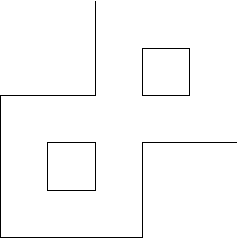
\includegraphics[width=0.32\textwidth]{sample1}~
	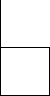
\includegraphics[width=0.07\textwidth]{sample2}~
	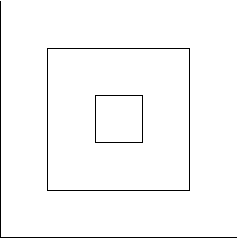
\includegraphics[width=0.32\textwidth]{sample3}~
	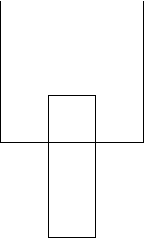
\includegraphics[width=0.19\textwidth]{sample4}
	\caption{Drawings of the four sample test cases.}
\end{figure}
